
%(BEGIN_QUESTION)
% Copyright 2006, Tony R. Kuphaldt, released under the Creative Commons Attribution License (v 1.0)
% This means you may do almost anything with this work of mine, so long as you give me proper credit

Draw schematic diagrams for the following RTDs:

$$\includegraphics[width=15.5cm]{i00404x01.eps}$$

Then, show how each type of RTD would connect to the input terminals of an RTD-input temperature transmitter.  Note how each transmitter is configurable for different types of RTDs, the different RTD types being shown symbolically on the face of the transmitter:

$$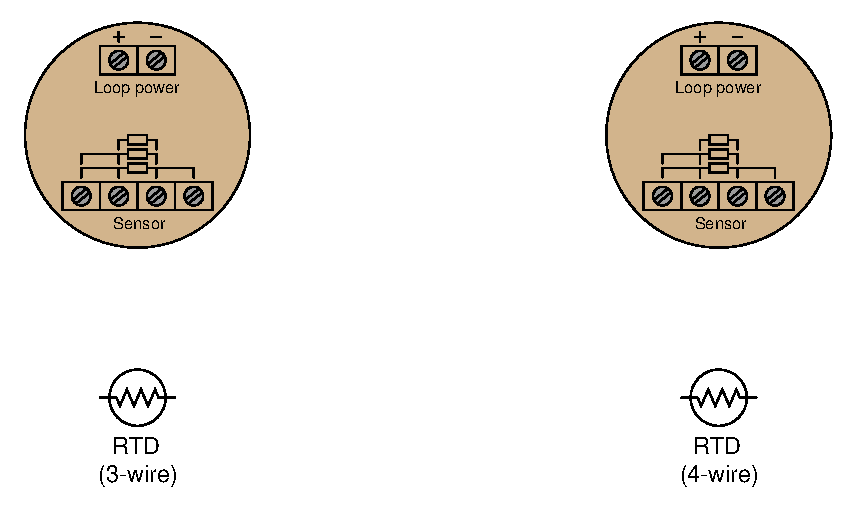
\includegraphics[width=15.5cm]{i00404x02.eps}$$

\vskip 20pt \vbox{\hrule \hbox{\strut \vrule{} {\bf Suggestions for Socratic discussion} \vrule} \hrule}

\begin{itemize}
\item{} What do common colors represent for RTD lead wires?  
\item{} What advantage is there to a four-wire RTD over a three-wire RTD to justify the extra expense and connections required for the fourth wire?
\item{} Interpret the meaning of the box-shaped resistor symbols found on the faces of the RTD temperature transmitters.  Do these symbols represent what gets connected to the terminals of the transmitter, or do they represent what is already built inside the transmitter?
\item{} Is it possible to connect a four-wire RTD to a temperature transmitter intended for use with three-wire RTDs?  How about connecting to a temperature transmitter intended for two-wire RTDs?
\item{} How will the temperature measurement be affected if one of the ``sense'' wires breaks open on the 4-wire RTD?
\item{} How will the temperature measurement be affected if one of the ``excitation'' wires breaks open on the 4-wire RTD?
\end{itemize}

\underbar{file i00404}
%(END_QUESTION)





%(BEGIN_ANSWER)

$$\includegraphics[width=15.5cm]{i00404x03.eps}$$

%(END_ANSWER)





%(BEGIN_NOTES)


%INDEX% Measurement, temperature: RTD

%(END_NOTES)


